\section{Concurrency}

Go は言語のコア機能の一部として並行処理機能を提供します。

ここでは goroutine と channel の概要とそれらを使って
さまざまな並行処理を実装する方法について説明します。

\subsection{Goroutines}
\textbf{goroutine} (ゴルーチン)は、Goのランタイムに管理される軽量なスレッドです。

\begin{lstlisting}[numbers=none]
go f(x, y, z)
\end{lstlisting}
と書けば、新しいgoroutineが実行されます。

\begin{lstlisting}[numbers=none]
f(x, y, z)
\end{lstlisting}
\texttt{f} , \texttt{x} , \texttt{y} , \texttt{z} の
評価は、実行元(current)のgoroutineで実行され、 
\texttt{f} の実行は、新しいgoroutineで実行されます。

goroutineは、同じアドレス空間で実行されるため、共有メモリへのアクセス
は必ず同期する必要があります。 \texttt{sync} パッケージは同期する際
に役に立つ方法を提供していますが、別の方法があるためそれほど必要ありま
せん。 (次のスライドで説明します)
\lstinputlisting[caption = goroutines.go]{goroutines.go}
\lstinputlisting[caption = goroutines.run,numbers=none]{goroutines.run}

\subsection{Channels}
チャネル( Channel )型は、チャネルオペレータの \texttt{<-} を
用いて値の送受信ができる通り道です。

\begin{lstlisting}[numbers=none]
ch <- v    // (1)
v := <-ch  // (2)
\end{lstlisting}
(データは、矢印の方向に流れます)
\begin{description}
\item[(1)] \texttt{v} をチャネル \texttt{ch} へ送信する
\item[(2)] \texttt{ch} から受信した変数を \texttt{v} へ割り当てる
\end{description}

マップとスライスのように、チャネルは使う前に以下のように生成します:

\begin{lstlisting}[numbers=none]
ch := make(chan int)
\end{lstlisting}

通常、片方が準備できるまで送受信はブロックされます。これにより、
明確なロックや条件変数がなくても、goroutineの同期を可能にします。

サンプルコードは、スライス内の数値を合算し、2つのgoroutine間で
作業を分配します。 両方のgoroutineで計算が完了すると、最終結果
が計算されます。
\lstinputlisting[caption = channels.go]{channels.go}
\lstinputlisting[caption = channels.run,numbers=none]{channels.run}

\subsection{Buffered Channels}
チャネルは、 \textbf{バッファ} ( buffer )として使えます。
バッファを持つチャネルを初期化するには、 \texttt{make} の
2つ目の引数にバッファの長さを与えます:

\begin{lstlisting}[numbers=none]
ch := make(chan int, 100)
\end{lstlisting}
バッファが詰まった時は、チャネルへの送信をブロックします。
バッファが空の時には、チャネルの受信をブロックします。

バッファが詰まるようにサンプルコードを変更し、何が起きるのかを見てみてください。
\lstinputlisting[caption = buffered-channels.go]{buffered-channels.go}
\lstinputlisting[caption = buffered-channels.run,numbers=none]{buffered-channels.run}

\subsection{Range and Close}
送り手は、これ以上の送信する値がないことを示すため、
チャネルを \texttt{close} できます。 受け手は、
受信の式に2つ目のパラメータを割り当てることで、
そのチャネルがcloseされているかどうかを確認できます:

\begin{lstlisting}[numbers=none]
v, ok := <-ch
\end{lstlisting}
受信する値がない、かつ、チャネルが閉じているなら、
\texttt{ok} の変数は、 \texttt{false} になります。

ループの \texttt{for i := range c} は、チャネルが
閉じられるまで、チャネルから値を繰り返し受信し続けます。

\textbf{注意}: 送り手のチャネルだけをcloseしてください。
受け手はcloseしてはいけません。 もしcloseしたチャネルへ
送信すると、パニック( panic )します。

\textbf{もう一つ注意}: チャネルは、ファイルとは異なり、
通常は、closeする必要はありません。 closeするのは、これ
以上値が来ないことを受け手が知る必要があるときにだけです。
例えば、 \texttt{range} ループを終了するという場合です。
\lstinputlisting[caption = range-and-close.go]{range-and-close.go}
\lstinputlisting[caption = range-and-close.run,numbers=none]{range-and-close.run}

\subsection{Select}
\texttt{select} ステートメントは、goroutineを複数の通信操作で待たせます。

\texttt{select} は、複数ある \texttt{case} のいずれかが
準備できるようになるまでブロックし、準備ができた \texttt{case} を
実行します。 もし、複数の \texttt{case} の準備ができている場合、
\texttt{case} はランダムに選択されます。
\lstinputlisting[caption = select.go]{select.go}
\lstinputlisting[caption = select.run,numbers=none]{select.run}

\subsection{Default Selection}
どの \texttt{case} も準備ができていないのであれば、
\texttt{select} の中の \texttt{default} が実行されます。

ブロックせずに送受信するなら、 \texttt{default} の \texttt{case} を使ってください:

\begin{lstlisting}[numbers=none]
select {
case i := <-c:
    // use i
default:
    // receiving from c would block
}
\end{lstlisting}
\lstinputlisting[caption = default-selection.go]{default-selection.go}
\lstinputlisting[caption = default-selection.run,numbers=none]{default-selection.run}

\subsection{Exercise: Equivalent Binary Trees}
同じ数列を保持するような、形の異なる二分木( binary tree )は多く存在し得ます。
例えば、ここに数列 1, 1, 2, 3, 5, 8, 13 を保持する2つの二分木があります。

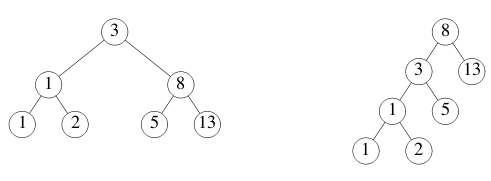
\includegraphics[width=10cm]{tree.png}

2つの二分木が同じ数列を保持しているかどうかを確認する機能は、多くの言語においてかなり複雑です。

シンプルな解決方法を記述するために、Goの並行性( concurrency )とチャネルを利用してみます。

例では、型を以下のように定義している \texttt{tree} パッケージを利用します:

\begin{lstlisting}[numbers=none]
type Tree struct {
    Left  *Tree
    Value int
    Right *Tree
}
\end{lstlisting}

1. \texttt{Walk} 関数を実装してください。

2. \texttt{Walk} 関数をテストしてください。

関数 \texttt{tree.New(k)} は、値( \texttt{k}, \texttt{2k}, \texttt{3k}, ..., \texttt{10k} )
をもつ、ランダムに構造化 (しかし常にソートされています) した二分木を生成します。

新しいチャネル \texttt{ch} を生成し、 \texttt{Walk} を動かしましょう:

\begin{lstlisting}[numbers=none]
go Walk(tree.New(1), ch)
\end{lstlisting}

そして、そのチャネルから値を読み出し、10個の値を表示してください。 それは、 1, 2, 3, ..., 10 という表示になるでしょう。

3. \texttt{Same} 関数を実装してください。 \texttt{t1} と \texttt{t2}
が同じ値を保存しているどうかを判断するため、 \texttt{Walk} を使ってください。

4. \texttt{Same} 関数をテストしてください。

\texttt{Same(tree.New(1), tree.New(1))} は、 \texttt{true} を
返すように、 \texttt{Same(tree.New(1), tree.New(2))} は、 \texttt{false} を
返すようにします。

\texttt{Tree} のドキュメントは
こちら(https:\//\//godoc.org\//golang.org\//x\//tour\//tree\#Tree) です。



\lstinputlisting[caption = exercise-equivalent-binary-trees.go]{exercise-equivalent-binary-trees.go}
% \lstinputlisting[caption = exercise-equivalent-binary-trees.run,numbers=none]{exercise-equivalent-binary-trees.run}

\subsection{sync.Mutex}
チャネルが、goroutine間で通信するための素晴らしい方法であることを見てきました。

しかし、通信が必要ない場合はどうでしょう? コンフリクトを避けるために、
一度に1つのgoroutineだけが変数にアクセスできるようにしたい場合はどうでしょうか?

このコンセプトは、排他制御( mutual exclusion )と呼ばれ、
このデータ構造を指す一般的な名前は mutex (ミューテックス)です。

Goの標準ライブラリは、排他制御を\texttt{sync.Mutex}と次の二つのメソッドで提供します:
\begin{description}
\item \texttt{Lock}
\item \texttt{Unlock}
\end{description}
\texttt{Inc} メソッドにあるように、 \texttt{Lock} と \texttt{Unlock} で
囲むことで排他制御で実行するコードを定義できます。

\texttt{Value} メソッドのように、mutexがUnlockされることを保証するために
\texttt{defer} を使うこともできます。
\lstinputlisting[caption = mutex-counter.go]{mutex-counter.go}
\lstinputlisting[caption = mutex-counter.run,numbers=none]{mutex-counter.run}

\subsection{Exercise: Web Crawler}
この演習では、ウェブクローラ( web crawler )を並列化するため、
Goの並行性の特徴を使います。

同じURLを2度取ってくることなく並列してURLを取ってくるように、 
\texttt{Crawl} 関数を修正してみてください(注1)。

\textbf{補足}: 工夫すれば \texttt{Crawl} 関数のみの修正
で実装できますが、無理に \texttt{Crawl} 関数内部に収める必要はありません。

\textbf{ひとこと}: mapにフェッチしたURLのキャッシュを保持できますが、
mapだけでは並行実行時の安全性はありません!
\lstinputlisting[caption = exercise-web-crawler.go]{exercise-web-crawler.go}
% \lstinputlisting[caption = exercise-web-crawler.run,numbers=none]{exercise-web-crawler.run}

\subsection{Where to Go from here...}
Goをインストール することで、Go言語を始めることができます。

Goをインストールしたなら、 Goのドキュメント は、 次に参考にする
にはとても良いものです。 ここにはリファレンスやチュートリアル、ビデオなどがあります。

Goのコードの構成や、動かし方を学ぶためには、 この
動画(https:\//\//www.youtube.com\//watch?v=XCsL89YtqCs)を見てください。
また、 How to Write Go Code を読んでください。

もし、標準ライブラリに関してヘルプが必要なら、 パッケージリファレンス を見てください。 言語自身に関してのヘルプは、 Go言語仕様 がとても参考になります。

Goの並行性のモデルについてもっと調べてみたいなら、 Go Concurrency Patterns (slides) や、 Advanced Go Concurrency Patterns (slides) を見たり、 codewalk: Share Memory by Communicating を読んでみてください。

Webアプリケーションをはじめてみるなら、 A simple programming environment (slides) を見たり、 チュートリアル: Writing Web Applications を読んでみてください。

First Class Functions in Go では、Goの関数型の興味深い側面を教えてくれます。

Go Blog には、Goに関する素晴らしい記事の多くのアーカイブがあります。

もちろん、 golang.org も見てください。

翻訳: @atotto